\documentclass{article}
\usepackage{graphicx}
\usepackage{outlines}
\usepackage{helvet}
\usepackage{microtype}

\renewcommand{\familydefault}{\sfdefault}
\title{BIOL BC3308: Independent Research Project}

\begin{document}

\maketitle{}

\section*{Deadlines}
\textbf{April 4, 12:59p: }Presentation 1 on Canvas\\
\textbf{April 25, 12:59p:} Presentation 2 on Canvas\\
\textbf{May 5, 12:59p:} Written component and code on Canvas

\section*{Overall goal} Conduct an independent research project to demonstrate your command of important microbial concepts, genomics, and bioinformatic analyses.

\section*{Ownership} All research being conducted in this assignment is novel. In addition to your grade on this project, if any of your findings contribute to ongoing research in the lab, you will be credited in the form of co-authorship on all resulting manuscripts.

\section*{Custom project policy} Custom projects are allowed and encouraged. To ensure fairness, we will need to work together to design a modified grading rubric, keeping it as close to the base rubric as possible. For feasibility, I will also require a project proposal following these guidelines:
\begin{outline}
    \1 Deadline: March 28, 2023, at 11:59 PM
    \1 State your research question and hypothesis.
    \1 Provide a list of at least 3 relevant papers + 1 sentence each describing their relevance to your project.
    \1 Produce a non-binding sketch of your methods, taking care to highlight how this departs from the default project and the course materials.
    \1 Suggest a contingency plan: what will you do if you can't get your data, if your pipeline fails, if your results are underwhelming, et cetera?
\end{outline}

\section*{Background} There are billions of bacterial strains and species inhabiting virtually every unique environment niche on this earth. Within these bacterial communities, plasmids spread rapidly and abundantly between cells through a process known as horizontal gene transfer (HGT), endowing certain strains with pathogenic traits. Some plasmids have been shown to be more widely disseminated than others, known as epidemic plasmids. Moreover, only some strains that come into contact with these epidemic plasmids are able to propagate it, ultimately causing infectious diseases. To understand the context surrounding this project, read the following three background papers:
\begin{itemize}
    \item \texttt{Andersson\_2020}
    \item \texttt{Dunn\_2019}
    \item \texttt{Mathers\_2015}
\end{itemize}

\section*{Project overview}
The Lopatkin lab studies HGT of plasmids to understand the broad overarching question:  Why are some plasmids and strains more successful than others? One project in the lab asks the specific question: what genetic features of a plasmid make it difficult to acquire through HGT? To answer this question, we have obtained and sequenced 39 representative clinical plasmids. In parallel, we have measured the difficulty of acquiring each of these plasmids, which is termed the plasmid cost. These results are shown in Figure 1 below and file \texttt{Summary\_table\_by\_plasmids.xlsx} on Canvas. As you can see, these plasmids exhibit a range of costs, from not costly ($\leq 1$) to highly detrimental ($>1$). We are currently in the process of closely inspecting each plasmid sequence to identify genetic determinants that are predictive of these measured costs. Our objective is to use bioinformatic analysis to generate hypotheses that can be tested experimentally in the lab---and you can help us! 

\begin{figure}
    \centering
    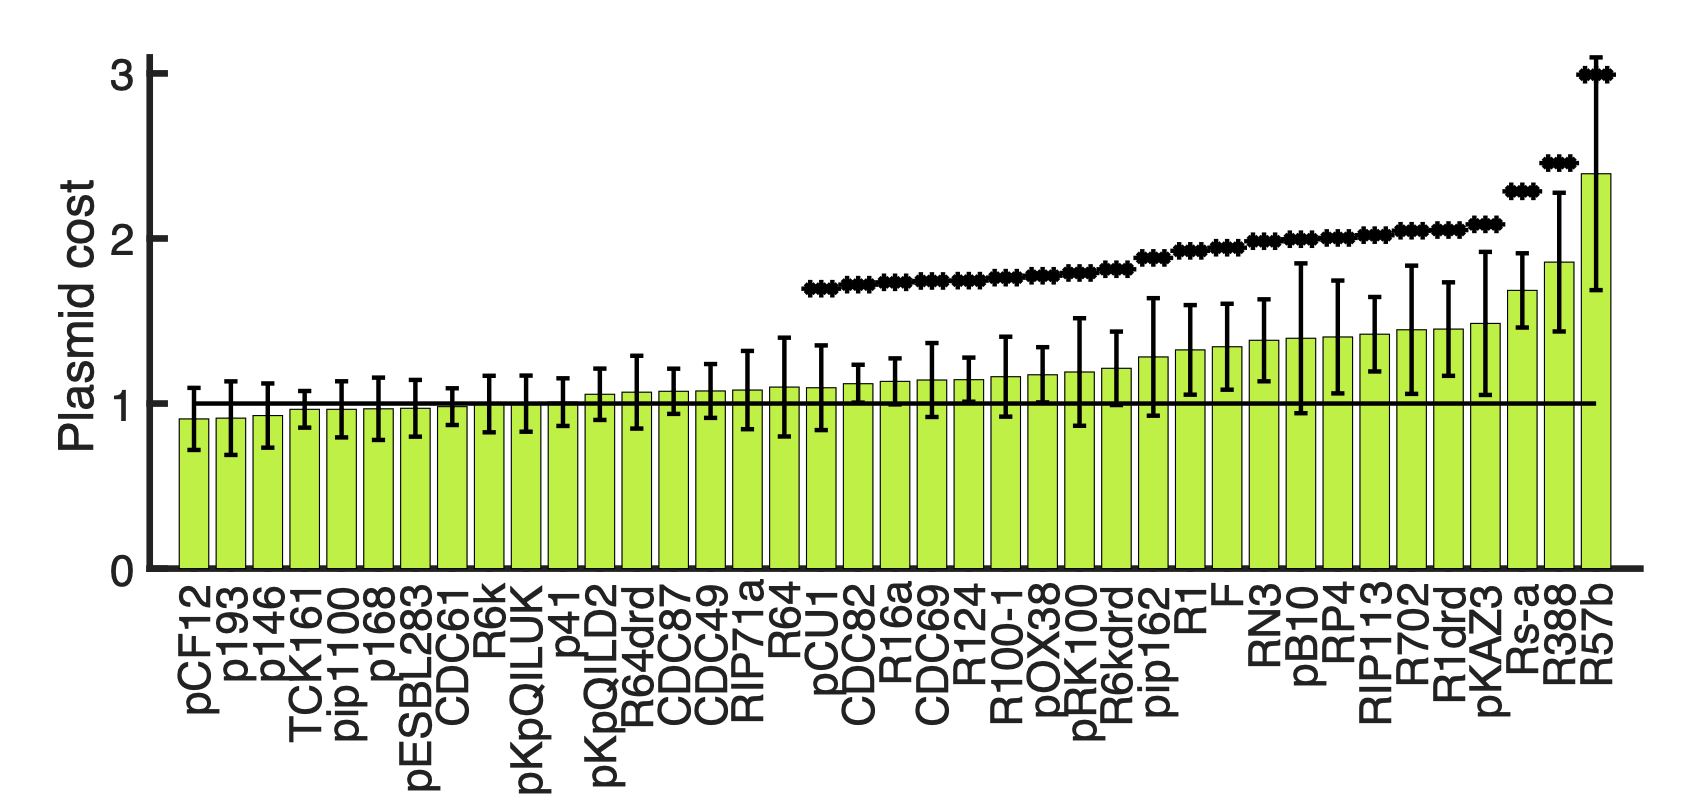
\includegraphics[width=\textwidth]{final_assignment_figs/final_assignment_fig1.png}
    \caption{Plasmid costs. Plasmid costs are measured by quantifying the growth defect in a bacterial cell that has recently acquired a plasmid compared. A value equal to 1 indicates no cost associated with acquiring the plasmid. Values greater than 1 indicate an increasingly difficult ability to acquire the plasmid. The x-axis is unique plasmids, and the y-axis is the cost for each. In this case, R57b is the most costly and pCF12 is the least costly plasmid. Stars indicate statistically significant cost. In other words, plasmid pCU1 is the first plasmid to show a statistically significant cost. Data generated by Hannah Prensky, Mehrose Ahmad, Shahd ElNaggar, and Maya Fabozzi.}
    \label{fig:fig1}
\end{figure}

\section*{Data provided on Canvas}
These files are located in \texttt{Files/Final\_project}:
\begin{enumerate}
    \item \texttt{proteins.fasta}: This is a multi-fasta file containing all representative protein sequences for the genes of interest. Find yours and save to a separate file.
    \item \texttt{Summary\_table\_by\_plasmids.xlsx}: Metadata for all plasmids in Figure \ref{fig:fig1} The columns include the following information:
    \begin{itemize}
        \item \textbf{Plasmid:} Name of each plasmid
        \item \textbf{INC:} Incompatibility group of the plasmid
        \item \textbf{cost\_av:} Average plasmid cost from all experimental replicates
        \item \textbf{cost\_std:} Standard deviation of plasmid cost from all experimental replicates
        \item \textbf{cost\_bin:} Binary indication of whether or not the plasmid has a statistical cost
        \item \textbf{p\_value\_corrected:} P-value indicating the statistical significance corresponding to \textbf{cost\_bin}
    \end{itemize}
    \item \texttt{Fastas/}: A folder containing the fasta files for each plasmid in our dataset
    \item \texttt{Papers/}: A folder containing pdfs of all reference papers below. This is a start point for your literature search
\end{enumerate}

\section*{Gene assignments}
\begin{table}[h!]
    \centering
    \begin{tabular}{|c|c|}
        \hline
        \textbf{Gen} &	\textbf{Assignment}\\
        \hline
        \textit{traD}	& Kayla\\
        \textit{psiB}	& Michelle\\
        \textit{trbB}	& Kaitlyn\\
        \textit{traG}	& Kaylene\\
        \textit{ssb}	& Cindy\\
        \textit{traW}	& Sylvie\\
        \textit{traT}	& Sophia\\
        \hline
    \end{tabular}
    \label{tab:assignments}
\end{table}

\section*{Research questions}
You will each conduct a bioinformatic analysis to answer two research questions: 
\begin{enumerate}
    \item For the single gene assigned above, is $\langle$your assigned gene$\rangle$ potentially important in determining the cost of a plasmid? Note that not every gene is on every plasmid. You will focus on three aspects of your gene:
    \begin{enumerate}
        \item Nucleotide or protein sequence 
        \item Intergenic nucleotide region upstream of your gene
        \item Genetic context surrounding the gene
    \end{enumerate}
    \item The second is an extension of (1) and investigates more generally whether plasmids with similar cost phenotypes share groups of genes and/or features. In this analysis, you will be responsible for defining the specific research question. A default framework is provided, but can be expanded and/or modified according to individual interests.

\end{enumerate}

\section*{Project details}
\begin{outline}[enumerate]
\1 \textbf{Research question 1:} Here you are assessing whether your assigned gene will likely be important in determining the plasmid cost. The order you take to accomplish the requirements below is up to you, but it must include the following. 
    \2 \textbf{Define a hypothesis:} Search the literature to understand your gene. Based on this knowledge, the provided data, and the research question above, hypothesize whether you expect (i) your gene itself (ie the sequence), (ii) its expression level (ie promoter region), and/or (iii) its local context (ie the genes located upstream and/or downstream from it), to impact the cost? Why or why not?
    \2 \textbf{Bioinformatic approach:} Perform comparisons of your gene as it exists in the given plasmid sequences. Include the comparisons of i-iii above.
    \2 \textbf{Justification:} Justify both your hypothesis and approach. For the latter, include a literature-based explanation for why you chose nucleotide or protein (i), how you will identify the intergenic region (ii) and appropriate genetic context to compare (iii). 
    \2 \textbf{Methods:} Generate a reproducible pipeline that answers i-iii above. This may include one or more Jupyter notebooks, pipelined shell + python scripts, and/or a Geneious workflow. See note1 for details.
    \2 \textbf{Visualization: }At least one figure or table of your results should be generated for each analysis in i-iii (multi-sequence alignment, phylogenetic tree, syntenic graph, etc.). See note2 for details.
    \2 \textbf{Interpretation: }Explain the main findings in each case (i-iii). Examine your results in the context of the gene function, the metadata, and research question. What predictions can you make, and how would you experimentally test it? Does your prediction make sense in the context of literature?
\1 \textbf{Research question 2:} Here you will use Prokka and Roary to analyze gene-set differences between different groups of plasmids. Exactly what question you ask is up to you, but again, it must be rigorous and reproducible. *Note that anyone interested in focusing on a different research question/approach using the same dataset is free to do so. Described below is the default; if you wish to focus on a different analysis, it must contain the same section*s a-f modified accordingly*
    \2 \textbf{Define a hypothesis: }Choose how you will segment the plasmids; this could be based on several aspects of the metadata, i.e., “high” vs. “low” cost, incompatibility group, etc. Based on these groupings, and the Roary documentation, formulate a specific research question and hypothesis. You can use all or only a subset of the plasmids, and any additional public resources as you would like (see note3). An example is included below:\\
    \textbf{Research question: }Do low-cost plasmids have unique core functions compare to high-cost plasmids? 
    \textbf{Hypothesis: }I hypothesize that the core genome of the 5 lowest cost plasmids will have a different set of enriched GO functions compared to the 5 highest cost plasmids.
    \2 \textbf{Bioinformatic approach:} Use concepts related to core- and pan-genomes to identify differences between your defined groups of plasmids
        \3 Run Roary to get the core genomes for each set of plasmids you chose
        \3 Use any of Roary’s set-difference functions to get the differences between core genomes of each set. How can you make this analysis more rigorous (ie is there a control you can run in parallel to assess your findings)? 
        \3 Use at least one manual tool(s) other than Prokka to annotate/enrich your gene sets to look for insights (genbank or ecocyc). For extra credit, use a command-line or automated tool/API (e.g., ecocyc, mob-typer, abricate, GO enrichment, etc.)
    \2 \textbf{Justification:} Justify your research question, hypothesis and approach. This should include why you chose to segment the plasmids using your chosen metric, literature support for your expectations, the purpose of including other public data if relevant, and why your annotation tools are appropriate.
    \2 \textbf{Methods:} Generate a reproducible pipeline that executes i-iii above. This may include one or more Jupyter notebooks, pipelined shell + python scripts, and/or a Geneious workflow. See note1 for details.
    \2 \textbf{Visualization:} At least two figures of your results should be generated; this could include phylogenetic trees, heatmaps, GO results, alignments, etc. Feel free to use any tools in any language (R, Python, Excel, etc.), or online tools to do so.
    \2 \textbf{Interpretation:} Explain your findings in the context of your hypothesis/expectations and relevant literature. Describe any experiments you’d like to perform to verify/dismiss your findings. For example, some components could be: Do you see strong differences in gene types between the two plasmid groups?  What are the functions of the genes that are common/different?  Are there any functionally-enriched groups that these genes encode?
\end{outline}

\section*{Submission components}
\begin{outline}[enumerate]
    \1 \textbf{(60 pt) Presentation 1:} A timed 10-12 minute powerpoint presentation. Half of your presentation should be focused on research question 1, and the second half on research question 2. For both, you should include the following (covering parts a-c above):
        \2 State the specific research question and your hypothesis
        \2 Describe your proposed bioinformatics approach
        \2 Justify your hypothesis, research question (if necessary), and approach using literature and data
    \1 \textbf{(60 pt) Presentation 2:} A timed 13-15 minute powerpoint presentation. This should summarize your main results from both research questions. You can split the presentation in half again if you wish, or dedicate more time to one or the other based on what you deem to be the most important results. It should include the minimum for each question:
        \2 Briefly re-state the research question
        \2 Briefly re-state the hypothesis/your expectations
        \2 Clearly state your main results
        \2 Include at least one representative visual output
        \2 The majority of the time should focus on the interpretation of your results in the context of data and literature, and should clearly demonstrate an understanding of the data, the analysis, and any potential limitations. Do you feel confident in your results to suggest experimental follow-up? If so, what do you propose? If not, why, and what additional data/information would you want to be able to make any concrete statements?
    \1 \textbf{(80pt) Written component:} One word document for each research question. Each document should summarize the results for each respective research question. In each document, please include the following section*s:
        \2 \textbf{Background and hypothesis:} include any relevant context and literature sources that you used to generate your expectations. Any citation format is accepted.
        \2 \textbf{Methods:} Describe the pipeline and tools that you used. This should be sufficiently detailed so that I can reproduce the results entirely.
        \2 \textbf{Results and discussion:} Include your visualizations as figures, as well as interpretation and justification of your methods/results as outlined in each question above.
    \1 \textbf{(100 pt) All associate scripts and functions (or Geneious workflows):} Everything should be sufficiently commented and should be able to run on my computer (including anything required to create environments locally).
\end{outline}

\section*{Papers}
\begin{enumerate}
    \item Fernandez-Lopez, R., de Toro, M., Moncalian, G., Garcillan-Barcia, M. P. \& de la Cruz, F. Comparative Genomics of the Conjugation Region of F-like Plasmids: Five Shades of F. Front. Mol. Biosci. 3, (2016).
    \item Zatyka, M. \& Thomas, C. M. Control of genes for conjugative transfer of plasmids and other mobile elements. FEMS microbiology reviews 21, 291–319 (1998).
    \item Frost, L. S. \& Koraimann, G. Regulation of bacterial conjugation: balancing opportunity with adversity. Future Microbiology 5, 1057+-1057+ (2010).
    \item Bischof, K. et al. Regulation of R1 Plasmid Transfer by H-NS, ArcA, TraJ, and DNA Sequence Elements. Front. Microbiol. 11, 1254 (2020).
    \item Cox, K. E. L. \& Schildbach, J. F. Sequence of the R1 plasmid and comparison to F and R100. Plasmid 91, 53–60 (2017).
    \item Audette, G. F., Manchak, J., Beatty, P., Klimke, W. A. \& Frost, L. S. Entry exclusion in F-like plasmids requires intact TraG in the donor that recognizes its cognate TraS in the recipient. Microbiology 153, 442–451 (2007).
    \item Althorpe, N. J., Chilley, P. M., Thomas, A. T., Brammar, W. J. \& Wilkins, B. M. Transient transcriptional activation of the IncI1 plasmid anti-restriction gene (ardA) and SOS inhibition gene (psiB) early in conjugating recipient bacteria. Mol Microbiol 31, 133–142 (1999).
\end{enumerate}

\section*{Notes}
\begin{outline}[enumerate]
\1 \textbf{Comparing the organization of genetic regions:} use any method (MAUVE, Geneious, Biopython synteny, assembling a table, etc.)
\1 \textbf{Viewing multi-sequence alignments:} there are many options here, but some include Geneious or online viewers like this one.
\1 Public resources:
    \2 \textbf{NCBI pathogens:} This database will allow you to search by microbial species. You can include columns of metadata by clicking on “choose columns”, and dragging over categories of interest (e.g., presence of genes, outbreak information, etc.). Once you have a curated metadata list, download the table and use the SRS identifier with fastq-dump.
    \2 \textbf{NARMS: }National surveillance data for antimicrobial resistant pathogens in diverse outbreaks. Explore to find the accession IDs.
    \2 \textbf{Pubmed and Google scholar:} Search using key words to find relevant literature
    \2 \textbf{Enterobase:} This database allows you to search by sequence type (ST), species, and other metadata features to curate a library of strains.
    \2 \textbf{Acquired antibiotic resistance genes:} \texttt{van\_Hoek\_2011}, \texttt{carattolli\_2009}
    \2 \textbf{Strain typing methods:} \texttt{Uelze\_2020}
\end{outline}

\section*{Final thoughts}
This is a time for you to be creative, exploratory, and thoughtful. There are a million and one ways to slices the data---you should be trying to collate all of the information that you learned through the first half of the semester, and demonstrate a comprehensive command of bioinformatic thought processes. Most importantly, have fun with it!

\end{document}
